%Papierformat
\documentclass[12pt,a4paper]{scrartcl}
%deutsche Silbentrennung
\usepackage[ngerman]{babel}
%Listen einrücken
\usepackage{enumitem}
%deutsche Umlaute
\usepackage[utf8]{inputenc}
%Trennung von deutschen Umlauten
\usepackage[T1]{fontenc}
%für Zitate
\usepackage[numbers,square]{natbib}
%Grafikpaket laden
\usepackage{graphicx}
%Grafik Floating einschränken
\usepackage{placeins}
%Referenzierung mit Name
\usepackage{titleref}
%Unterschritszeilen
\usepackage{tabularx}
%Verlinkung
\usepackage{hyperref}
%für url erkennung
\usepackage{url}

%\makeatletter
%\newcommand\footnoteref[1]{\protected@xdef\@thefnmark{\ref{#1}}\@footnotemark}
%\makeatother​

%Dokumentbeginn
\begin{document}

	%Festlegung des Zitatstyles - Harvardmethode: Abkuerzung Autor + Jahr
	\bibliographystyle{alphadin}

\begin{titlepage}
	%Eine mbox wird verwendet um Text zusammenzuhalten
	%vspace erzeugte die in Klammern angegebenen Zeilenabstände
	%baselineskip setzt zeilenabstand
   	\mbox{}\vspace{5\baselineskip}\\
   	%Schriftart und Größe als Attribut
   	\rmfamily\huge
   	%Mittige Textausrichtung (\centerline für eine Zeile)
   	\centering
   	%Das Argument erscheint in Kapitälchen (small capitals).
	\textsc{Security in Android}
	%Umbruch bezogen auf die Höhe des Kleinbuchstaben x in diesem Element * Faktor
	\\[3ex]
   	Seminararbeit
   	\rmfamily\Large
   	\vspace{1\baselineskip}\\
   	%Externes einbinden einer Textdatei
   	%\input{version.txt}\mbox{}
%	\vspace{3\baselineskip}\\
	Hochschule f"ur angewandte Wissenschaften W"urzburg-Schweinfurt
   	\vspace{5\baselineskip}\\
   	\rmfamily\Large
   	Kristoffer Schneider
   	\vspace{1\baselineskip}\\
   	%Heutiges Datum
   	\today
\end{titlepage}

	%Inhaltsverzeichnis
	\tableofcontents
	\newpage
	%Falls nötig...
	%Literaturliste im Inhaltsverzeichnis anzeigen
	%\addcontentsline{toc}{section}{Literatur}
	
	%Abbildungsverzeichnis
	\listoffigures
	\newpage

	\subsection{Android}
	Das Unternehmen Android wurde 2003 von Andy Rubin gegründet und wurde 2005 von
	Google aufgekauft. Seitdem hat Google und das Android Open Source Project
	(AOSP) die Weiterentwicklung des Systems übernommen. Zuletzt wurden die neuen
	Versionen jeweils von Google intern entwickelt und zum Release der Version der
	AOSP Community als Open-Source bereitgestellt. Das Betriebssystem wird in den
	meisten Fällen von den Smartphone Herstellern oder Entwicklerteams noch weiter
	angepasst, bevor es für die einzelnen Geräte bereitgestellt wird.\\
	Basis für das Betriebssystem ist ein modifizierter Linux-Kernel und eine Java
	Virtual Machine (JVM) \cite{ArtDalvik}. Bis einschließlich Version 4.4 wurde
	hierfür die Dalivk Runtime und für alle neueren Versionen die Android Runtime
	(ART) verwendet. Jede App l"auft in einer eigenen Instanz der entsprechenden
	Runtime und in einer Sandbox. Oberhalb der JVM sind die meisten Komponenten in
	Java implementiert.
	\begin{figure}[h]
		\centering
		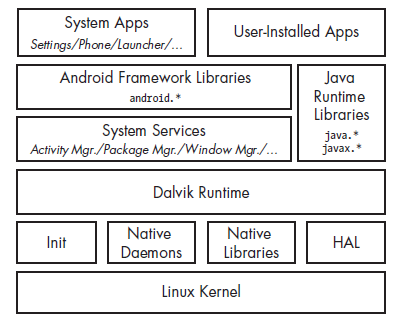
\includegraphics[width=0.7\linewidth]{android_pages/graphics/architektur_android_.png}
		\caption{Die Android Architektur \protect\cite[S. 2]{Elenkov2014} }
		\label{fig:architektur_android}
	\end{figure}
	\\\\
	\textbf{Die Dalvik- und Android Runtime}\\
	Ein grundsätzlicher Unterschied zwischen einer klassischen JVM, wie sie auf
	dem Desktop und anderen Geräten zum Einsatz kommt, und einer Runtime die auf
	Android läuft ist der, dass auf Android die Runtime auf einer Register-
	anstatt auf einer Stackmaschine basiert \cite{DalvikBytecode}. Somit
	unterscheidet sich der Bytecode zwischen den Plattformen. Eine
	Registermaschine bringt mehrere Vorteile mit. Unter anderem ist der Bytecode
	kleiner, was gerade mobilen Endgeräten entgegen kommt.
	Zusätzlich wird nicht mehr mit den üblichen \textit{jar}- und
	\textit{class}-Dateien, sondern mit einem eigenen Format namens \textit{.dex}
	gearbeitet \cite{DexFormat}. Dieses ist für den mobilen Einsatz optimiert.\\
	Die Dalvik Runtime stammt noch aus dem ursprünglichen Android Projekt und
	ähnelt einer klassischen JVM noch sehr. Sie interpretiert Bytecode zur
	Laufzeit und ist in der Lage oft genutzten Code zur Laufzeit zu kompilieren
	(\textit{Just-in-time-Compilation, kurz: JIT}).
	Die größte Änderung mit dem Umstieg auf die Android Runtime ist, dass nun
	vorkompilierter Programmcode (\textit{Ahead-Of-Time-Compilation}, kurz:
	\textit{AOT}) genutzt wird. Der Hintergrundgedanke dieser Veränderung ist,
	dass dadurch die Performance deutlich verbessert wird. Allerdings ist nativ
	kompilierter Code größer als Bytecode, wodurch wiederum mehr Speicher auf den
	Geräten benötigt wird. Da Android auf vielen verschiedenen Hardware
	Plattformen ausführbar sein muss und der native Code plattformabhängig ist,
	wird der Bytecode während der Installation in Nativen kompiliert.\\
	Durch das Nutzen von Java wird Exploits, welche auf Basis von Bufferoverflows
	arbeiten, entgegen gewirkt, da Java die Speicherzugriffe überprüft und bei
	Überläufen eine Exception wirft, was den Abbruch der auslösenden Operation als
	Folge hat. Dieser Schutz ist allerdings nur unter der Nutzung von
	Java-Programmcode vorhanden und nicht wenn nativer, z.B. durch den Einsatz des
	Java-Native-Interfaces (\textit{JNI}), genutzt wird.

	\newpage
	
	\subsection{Android}\label{sec:app-android}
	\begin{quote}
	Android apps are written in the Java programming language. The Android SDK tools compile your code - along with any data and resource files - into an APK: an \textit{Android package}, which is an archive file with an .apk suffix. One APK file contains all the contents of an Android app and is the file that Android-powered devices use to install the app.\cite{AndroidApp}
	\end{quote}
	
\begin{flushleft}
	Applikationen werden zumeist in Java oder C/C++ geschrieben; selten kommen auch andere JVM-Sprachen zum Einsatz.
	Eine Android App besteht im Kern unter anderem aus zwei wichtigen Teilen: den eigentlichen Programmkomponenten und einer Manifest Datei (AndroidManifest.xml).\\
\end{flushleft}
	\subsubsection{Programmkomponenten}
	Als Programmkomponenten können unter anderem vorkommen:
	\begin{itemize}\itemsep0pt
		\item Activities - stellen die Benutzeroberfläche dar
		\item Services - kann im Hintergrund laufen, auch wenn die App minimiert ist
		\item Content Provider - stellt Daten für die eigene und evtl für andere Apps zur Verfügung
		\item Broadcast Receiver - um Systemweite Benachrichtigungen zu empfangen (z.B dass ein Download beendet wurde)
	\end{itemize}
	\subsubsection{Manifest-Datei}
	In der Manifest-Datei werden Eigenschaften der App definiert. Darunter zählen beispielsweise:
	\begin{itemize}\itemsep0pt
		\item Name der App
		\item Ziel SDK-Versionen
		\item Versionsnummer
		\item optional eine UserId (Kapitel \ref*{sec:BasisRechteSystem})
		\item Permissions (Kapitel \ref*{sec:SandBoxingNPermissions})
		\item Startpunkt der Applikation
	\end{itemize}
	\subsubsection{Signatur}
	Jede App muss signiert werden. Das hierfür benötigte Zertifikat kann sich jeder Entwickler selbst generieren und muss nicht durch eine Certification Authority (CA) beglaubigt werden. Dabei wird angeraten, dass ein Entwickler für all seine Apps dasselbe Zertifikat nutzt. Mithilfe der dadurch gegebenen Signatur wird eine \textit{Same-Origin-Policy} erschaffen, die bei jedem Update sicherstellt, dass dieses wirklich vom Entwickler der Applikation stammt und nicht durch Dritte eingebracht wurde.\\\\
	Hauptquelle für Anwendungen der Android Plattform ist der \textit{Google Play Store}. Mittlerweile gibt es allerdings auch andere vertrauenswürdige Quellen, z.B. Amazons \textit{App Shop}.
	
	\subsubsection{Entwicklung}
	Java als Programmiersprache bringt mehrere Vorteile mit sich. Mit die wichtigsten sind, dass Java leicht zu lernen ist, was sich entsprechend auch auf die Anzahl der Apps für Android niederschlägt. Auch gibt es eine große Anzahl an Entwicklungsumgebungen, die oftmals sogar kostenlos nutzbar sind.\\
	Dass Apps somit schnell programmiert werden können, kann allerdings auch ein Nachteil sein, z.B. wenn Entwickler aufgrund von Unwissen Nutzerdaten nicht korrekt schützen, oder sogar versehentlich eine Sicherheitslücke zur Verfügung stellen.
	\newpage
	
	\section{Sicherheitsaspekte der Android-Architektur}

	Bereits durch die Architektur des Betriebssystems, insbesondere durch die restriktive Rechtevergabe und das Sandboxing, wird versucht, ein möglichst sicheres System bereitzustellen. Ab Android Version 4.3 kommt zusätzlich noch \textit{Security-Enhanced Linux (SELinux)} zum Einsatz.\\
	Verschlüsselungen und Signaturen werden Hardwareseitig durch eine \textit{Trusted Execution Environment (TEE)} unterstützt. TEE stellt einen besonders geschützten Bereich auf dem Prozessor dar, auf dem nur berechtige Anwendungen ausgeführt werden können, wie beispielsweiße die Verifikation des Bootmediums und Verschlüsselungsverfahren. Die Implementierung ist dabei Prozessor Hersteller abhängig - auf ARM wird dabei, wie bei iOS, auf \textit{TrustZone}\cite{TEE_ARM} zurückgegriffen.
	
	\subsection{Verifikation der Bootmedien} \label{sec:VerifikationDerBootmedien}
	Um bereits bei Systemstart eine Veränderung oder Ersetzung der Paritionen zu erkennen, wurde mit Android 4.4 eine Boot Verification eingeführt. Das Verfahren basiert auf der Funktion dm-verity des Device Mappers, welcher im Linux Kernel zu finden ist. Da diese Überprüfung durch den Kernel ausgeführt wird, muss vor dem Start von dm-verity erst der Bootloader und die Boot-Partition selbst auf ihre Integrität überprüft werden.
	Die Verifikation des Bootloaders ist nur schwer möglich, daher wird hierbei auf eine Hardware basierende root-of-trust, hier auf Basis des TEE, gesetzt. \\
	
	\subsubsection{Integritätscheck durch den Bootloader}
	Grundsätzlich ist Implementierung des Bootloader und dessen Vorgehen stark Geräteabhängig, daher werde ich hier im Folgenden lediglich das prinzipielle Vorgehen, welches durch das AOSP unterstützt wird, erläutern.\\
	Um die Boot- und Recovery-Partition (\textit{/boot, /recovery}) zu validieren gibt es zwei Möglichkeiten. Ist auf den beiden Partition jeweils ein offizielles Images des Smartphone Herstellers, kann auf einen OEM Key zurückgegriffen werden. Dieser ist in einem read-only in der Hardware festgeschrieben und wird vom Hersteller des Systems - zumeist der Smartphone Hersteller - festgelegt. Sollte eine Veränderung des Images vorgenommen worden sein, egal ob bewusst durch den Nutzer oder durch Schadcode, ist dieses Vorgehen nicht mehr möglich. Um aber dennoch eine Modifikation durch den Nutzer grundsätzlich zu ermöglichen, gibt es noch eine zweite Möglichkeit. Dabei wird auf ein, in der Paritionssignatur gespeichertes, Zertifikat zurückgegriffen.\\\\
	Um zu unterscheiden ob ein offizielles oder inoffizielles Image erwartet wird, kann der Bootloader zwischen zwei Status unterscheiden:\\
	
	\begin{itemize}\itemsep0pt
		\item LOCKED - das aktuelle Boot-Image ist ein offizielles und kann mittels OEM Key verifiziert werden
		\item UNLOCKED - das aktuelle Boot-Image wurde verändert, und kann daher nicht mit dem OEM Key veriiziert werden
	\end{itemize}
	
\begin{flushleft}
	Diese und andere Informationen sind zwischen verschiedenen Images weites gehend gleich und werden daher auf einer extra Partition gespeichert (zumeist \textit{/misc} oder \textit{/param}), welche somit im Falle eines Wechsel des Images nicht neu aufgesetzt werden muss.
\end{flushleft}
	 Wurde dies getan, wird beim Hochfahren immer eine Warnung ausgegeben, um den Nutzer darauf hinzuweisen, dass die Partition nicht mittels des festgeschrieben Keys verifiziert werden konnte. Daraus ergeben sich mehrere mögliche Zustände des Systems:\\\\
	
	\begin{figure}[h]
		\centering
		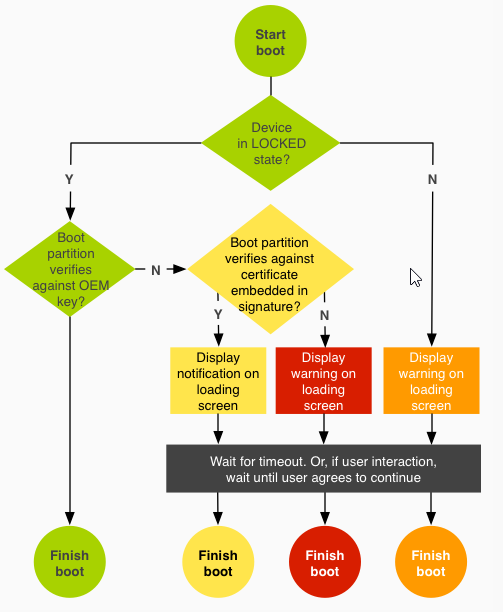
\includegraphics[width=0.7\linewidth, height=0.5\textheight]{android_pages/graphics/VerifiedBoot}
		\caption[Verified boot flow\protect\cite{VerifyingBoot}]{Verified boot flow\protect\cite{VerifyingBoot}}
		\label{fig:VerifiedBoot}
	\end{figure}
	
\begin{flushleft}
	Mit diesem Vorgehen wird auch die Integrität des Kernels sichergestellt, welcher in der \textit{/boot-} Partition abgelegt ist. Die Steuerung wird nach diesem Vorgang an den Kernel übergeben, welcher die Verifikation weiterer Partitionen übernimmt.\newline\\

	Um zu verhindern, dass Angreifer einfach den Bootloader manipulieren um an Daten heranzukommen, muss die Partition welche die Nutzerdaten beinhaltet (\textit{/userdata}) vor einer Veränderung an dem Bootsystem formatiert werden.
\end{flushleft}
	
	\subsubsection{Integritätscheck weiterer Paritionen}
	Weitere Integritätschecks werden von der Kernelfunktion dm-verity übernommen.
	dm-verity arbeitet mit einem SHA-256 Hash-tree, der wie folgt aufgebaut ist:\\
	Für jeden 4K Sektor auf der Parition wird ein Hashwert berechnet. Jeweils zwei dieser Werte werden wiederum zu einem Neuen verrechnet. Dies wird solange wiederholt, bis nur noch ein Hashwert, der \textit{root-hash}, übrig ist. Um nun die Integrität sicherzustellen wird dieser root-hash, mit einem bereits berechneten Soll-Wert verglichen. Sind diese identisch, ist die Parition integer.
	
	\begin{figure}[h]
		\centering
		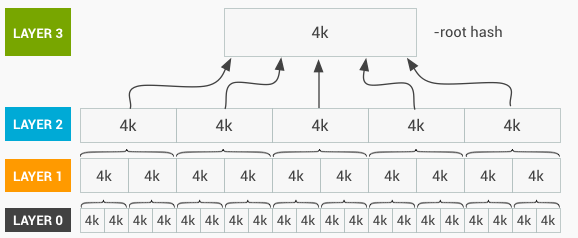
\includegraphics[width=0.7\linewidth]{android_pages/graphics/dm-verity-table}
		\caption[Aufbau des Hash-Trees]{Aufbau des von dm-verity erstellten Hash-Trees\protect\cite{VerifiedBoot}}
		\label{fig:dm-verity-table}
	\end{figure}
	
\begin{flushleft}
	Um Manipulationen am Soll-Wert zu unterbinden, wird der Hash-Tree und ein Salt mit einem RSA Schlüssel signiert. Der genutzte RSA Public Key wird in der Boot-Partition abgelegt. Der Hash-Tree und der Salt hingegen werden hinter dem letzten Datenblock auf die zu verifizierenden Partitionen geschrieben. Besonders geeignet ist dieses Verfahren für Read-Only Paritionen, wie die System-Partition welche das Betriebssystem beherbergt.\\
	Welche Paritionen mittels vm-verity auf ihre Integrität überprüft werden sollen, wird über einen Eintrag zu der jeweiligen Partition in der fstab-Datei festgelegt.
\end{flushleft}

	\subsection{Basis Rechtesystem}\label{sec:BasisRechteSystem}
	Von Linux wurde auch das Basis-Rechtesystem Übernommen, allerdings wird es leicht abgewandelt genutzt. Anstatt das ein Nutzer des Mobilsystems eine eindeutige User-ID (UID) zugewiesen bekommt, wird jede Applikation auf dem System als ein Nutzer angesehen und bekommt zur Installationszeit eine UID. Jeder Nutzer, und somit auch jede App, arbeitet grundsätzlich erst einmal nur innerhalb der ihm zugewiesenen virtuellen Maschine und dem damit verbundenen Dateisystem.\\\\
	Da es dennoch in vielen Fällen nötig ist, Daten zwischen verschiedenen Apps auszutauschen, gibt es mehrer Möglichkeiten dies zu tun. Die üblichen Wege wären Intends oder Contentprovider. Zusätzlich gibt es noch die Möglichkeit mehreren Apps dieselbe UID zuweisen zu lassen. Dies ist allerdings nur möglich, wenn die entsprechenden Applikationen mit dem selben Zertifikat signiert wurden und in deren Manifest Datei eine gemeinsame UID festgelegt wurde.
	Durch dieses Rechtesystem wird versucht sicherzustellen, dass kein Nutzerprogramm als \textit{root} ausgeführt wird.
	
	\subsection{Sandboxing und Permissions} \label{sec:SandBoxingNPermissions}
	Wie bereits erwähnt, laufen die Applikationen jeweils in ihrer eigenen Sandbox. Grundsätzlich ist die App damit in ihrer Ausführung auf ihren Bereich beschränkt und kann nicht mit anderen Prozessen und Daten ausserhalb interagieren. Dennoch ist es in den meisten Fällen sinnvoll mit Systemservices und Nutzerdaten zu interagieren, die nicht in der eigenen Sandbox verfügbar sind. 
	
	\subsubsection{Sandboxing}
	Das Sandboxing in Android basiert auf dem Rechtesystem des Linux-Kernels und der JVM. Prozesse eines Nutzer können nicht den Prozess eines anderen beeinflussen, noch auf dessen Arbeitspeicher oder internen Dateien zugreifen. Damit laufen die Nutzerprozesse jeweils isoliert von einander. Zusätzlich wird für die Ausführung von Bytecode eine JVM eingesetzt, welche auch nochmal eine Abstraktionsebene bereitstellt und den Einsatz von Exploits die auf einem Bufferoverflow basieren an verhindern soll.
	
	\subsubsection{Permissions im Detail}
	Um nun die bestehenden Zugriffsrechte erweitern zu können, müssen die entsprechenden Rechte (Permissions) in der Manifest Datei deklariert und angefordert werden. Zu Installationszeit werden diese Permissions dem Nutzer angezeigt und dieser wird gefragt, ob er den Rechtswünschen der App zustimmt oder nicht. Dabei gilt das \textit{Alles-Oder-Nichts-Prinzip}, d.h. entweder bekommt die Anwendung alle Rechte oder keine - was eine nicht Installation zur Folge hat. Des weiteren können die Berechtigungen nach der Installation nicht mehr angepasst werden.\\
	Oben genannte Berechtigungen sind beispielsweiße für Zugriffe auf externe Speichermedien oder auch die Kamera nötig. Dabei ist allerdings zu beachten, dass die Permissions zum Teil sehr grob definiert sind. Wodurch für den Nutzer nicht unbedingt erkenntlich ist, welche Informationen eine App warum abgreift und ob die App wirklich Gebrauch des Rechts macht.\\
	Anhand der folgenden Permission lässt sich die daraus resultierende Problematik gut erkennen:\\
	RECORD\_AUDIO Permission:
	\begin{quote}
	Allows an application to record audio \footnote{https://developer.android.com/reference/android/Manifest.permission.html\#RECORD\_AUDIO}
	\end{quote} 
	Dabei ist für den Nutzer nicht sichtbar, wann eine Aufnahme läuft, ausser die Applikation stellt dafür einen Hinweis bereit - wobei hier die Frage ist ob dieser auch wirklich verlässlich ist. Stellt die App einen Service bereit, kann ein solcher Mitschnitt auch im Hintergrund geschehen, und damit auch während eines Telefonats. Die einzige Chance RECORD\_AUDIO zur Laufzeit zu unterbinden ist, den Service bzw. die App über den Anwendungsmanager zu beenden.\\
	Ausnahmen für diese Problematik sind Module wie GPS, WLAN und Bluetooth. Diese kann der Nutzer des Geräts abschalten und damit den Zugriff darauf verweigern.
	Dennoch ist das Problem auf viele Permissions übertragbar.\\\\
%	Für die nächste Android Version, Android M, ist eine Verbesserung dieses Berechtigungssystems geplant und auch bereits vorgestellt worden. Es wird nun ermöglicht zur Laufzeit von Applikationen diesen Berechtigungen zu entziehen und freizugeben. Damit bekommt der Nutzer deutlich mehr Möglichkeiten, um seine Daten zu schützen. Allerdings wird es wohl kein Update für ältere Versionen geben, wodurch dort das Problem bestehen bleibt.
	Mit Android 4.3 (Kitkat) wurde eine versteckte Einstellungs-Activity namens \textit{App Ops} eingeführt. Darin konnte man einsehen welche App, wann welche Permission genutzt hat, und dieser einzelne Rechte zu entziehen und wieder zu erlauben. Diese Funktion konnte nur durch das Anlegen eines Activity Shortcuts und der direkten Verwendung in einer App genutzt werden. Leider wurde diese versteckte Einstellung aus den nächsten Versionen entfernt - bis Android M. \cite{HiddenActivity} \\
	Für Android M wurde mittlerweile angekündigt, dass eine derartige Einstellung nun fest mit eingebaut sein wird.\cite{AndroidMPermission}\\
	Allerdings wird es wohl kein Update für ältere Versionen geben, wodurch das Problem in diesen bestehen bleibt.
	
	\subsubsection{Besonderheit: Systemapps}
	Apps der System Hersteller können Rechte besitzen, die für normale Anwendungen nicht verfügbar sind, um Basis Apps und Services bereit zustellen. Hierfür werden alle Hersteller Applikationen mit sogenannten \textit{Publisher Keys} signiert.
	
	\subsection{SELinx in Android}
	Das \textit{Discretionary Access Control (DAC)} System des Linux Kernels lässt nur relativ grobe Einstellungen zu. Hat man beispielsweiße eine Applikation, die höhere Rechte für die Ausführung benötigt, so bekommt diese unter Nutzung von DAC oftmals noch zusätzliche Rechte, welche die App nicht haben sollte.\\
	Um dieses Problem zu beheben wird seit Android 4.4 zusätzlich zum DAC noch SELinux und dessen \textit{Mandatory Access Control (MAC)} System genutzt.\\	
	\begin{quote}
	SELinux operates on the ethos of default denial. Anything that is not explicitly allowed is denied.\cite{SELinuxAndroid}
	\end{quote}
	Dabei wird, sofern das DAC System einen Zugriff gewährt, das MAC System konsultiert und nur wenn dieses auch den Zugriff gewährt. Welche Rechte eine Applikation hat und welche nicht, wird unter SELinux in MAC Policies festgehalten. 
	
	Dabei sind zwei Nutzungsmodi zu unterscheiden. Während im \textit{permissive mode} Regelverstöße nur geloggt werden, wird im \textit{enforcing mode} die strikte Einhaltung erzwungen. In den Versionen 4.3 bis exklusive 5.0 war der \textit{enforcing mode} nicht überall in Nutzung. Dies änderte sich mit Version 5.0, seit dem läuft nur noch dieser Modus.
	
	\subsection{Verschlüsselung}
	\subsubsection{Datenträger Verschlüsselung}
	Mit Android 3.0 (Honeycomb) wurde die Möglichkeit eingeführt, die userdata-Partition zu vollständig verschlüsseln (Fulldisk Encryption - FDE). Basis der Verschlüsselung ist, wie bei der Verifikation der Partitionen (\ref{sec:VerifikationDerBootmedien}), eine Funktion des Device Mappers - dm-crypt. %Also Verschlüsselungsalgorithmus wird 
	
	\subsection{Sicherheit durch zentrale App Quelle}
	Dadurch, dass Apps für Android im Normalfall über den \textit{Google Play Store} verbreitet und von dort aus installiert werden, kann diese zentrale Quelle als weiterer Sicherheitsfaktor angesehen werde - zumindest bis zu einem gewissen Grad. Google hat bereits in der Vergangenheit Applikationen, welche Schadcode enthielten, aus dem Store entfernt. Zusätzlich dazu, ist per Default die Installation aus anderen Quellen, als dem Play Store, nicht möglich. Wodurch eine heimliche oder auch fehlerhafte Installation unterbunden werden soll. Sollte der Nutzer dennoch Anwendungen aus Drittquellen installieren wollen, beispielsweiße um Firmen interne Apps zu nutzen, kann der Nutzer diesen Schutz in den Einstellungen des Geräts deaktivieren.
	
	\newpage
	
	

\end{document}
